\documentclass[conference]{IEEEtran}
\usepackage{graphicx}
\usepackage{placeins}
\usepackage{hyperref}
\usepackage{subcaption}
\usepackage{eso-pic}
\usepackage{gensymb}
\usepackage{amssymb}
\usepackage{amsmath}


%\title{Predicting local street temperatures using crowd-source data and a machine learning approach. }
\date{\today}
%\usepackage[style=nature,backend=bibtex,doi=true,url=true]{biblatex}
%\bibliography{/usr/people/pagani/sharePrivateNetDrive/pagani/collaborations/UtrechtUniv/biblio}
%\graphicspath{{/usr/people/dirksen/reports/City_temperatures_figures/}}

\author{
	\IEEEauthorblockN{Andrea Pagani}
	\IEEEauthorblockA{De Bilt, Netherlands\\ Email: andrea.pagani@knmi.nl}}
\title{
	%\leavevmode\smash{\includegraphics[width=0.2\textwidth]{knmi}}\\
	Fog detection conditions from camera images using supervised and unsupervised learning.
}

\begin{document}
\maketitle

\section{Introduction}
Fog and mist are natural phenomena that are particularly dangerous for traffic and public safety due to the reduction of visibility. Fog is responsible for extreme accidents conditions involving tens to hundreds vehicles in a single accident location~\cite{hamilton2014hidden}. Compared to other meteorological phenomena (e.g., precipitation, cloud coverage), 
fog is quite difficult to forecast due to the several conditions in which fog can arise. For example, fog 
formation is influenced by the amount of precipitation and humidity in the ground, by the temperature 
difference between ground and  lower layers of the atmosphere touching the ground, by the absence of wind, by the 
presence of water basins in the surroundings their temperature of the water compared to the air. In particular, 
temperature difference between ground and air is usually more evident in specific moments in the day such as sunrise and sunset.
Given the particular conditions in which mist can arise, it can be a highly local phenomenon taking 
place in one small region and suddenly disappear in a region few kilometers away.

Therefore, given the complexity and the locality of this phenomenon, in this project the idea is to detect mist and fog conditions coming mainly from camera images rather than forecasting the 
presence of fog. In the Netherlands there is a high concentration of cameras to monitor the traffic along 
many of the highways in the country, this could be a good data source to use.

\section{Problem definition}
The goal is to recognize conditions of fog and mist from images. The identification of mist conditions 
is primarily based on the the picture; other features representing the meteorological conditions can also be used where available. Pictures can be taken in different locations, thus it cannot be 
implied the presence of any additional reference objects or recurrent patterns in the image in clear conditions. 
Furthermore, the main objective is to have a probability indicator for the chance that the image is foggy. 

		\begin{figure}[ht]
			\centering
			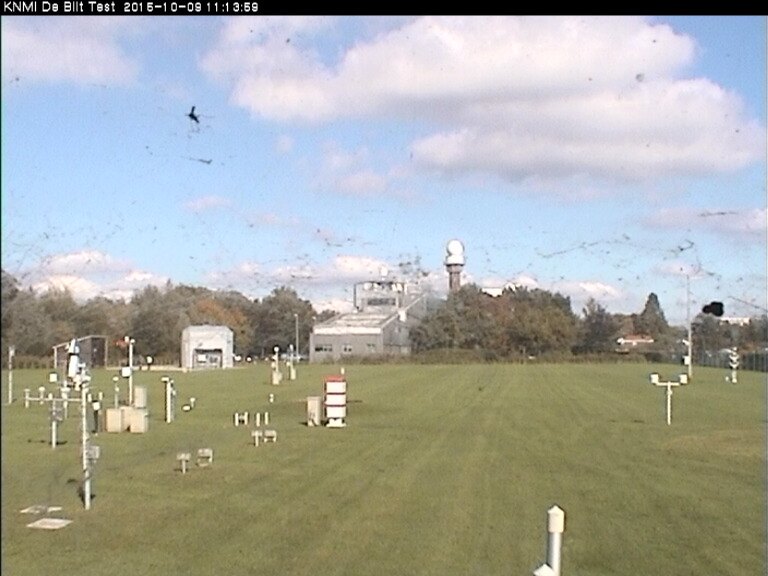
\includegraphics[width=0.22\textwidth]{Meetterrein_20151009_1110.jpg}	
			\caption{Measurement field at KNMI-De Bilt: clear conditions.}
			\label{fig:clear}
		\end{figure}
		
		
				\begin{figure}[ht]
			\centering
			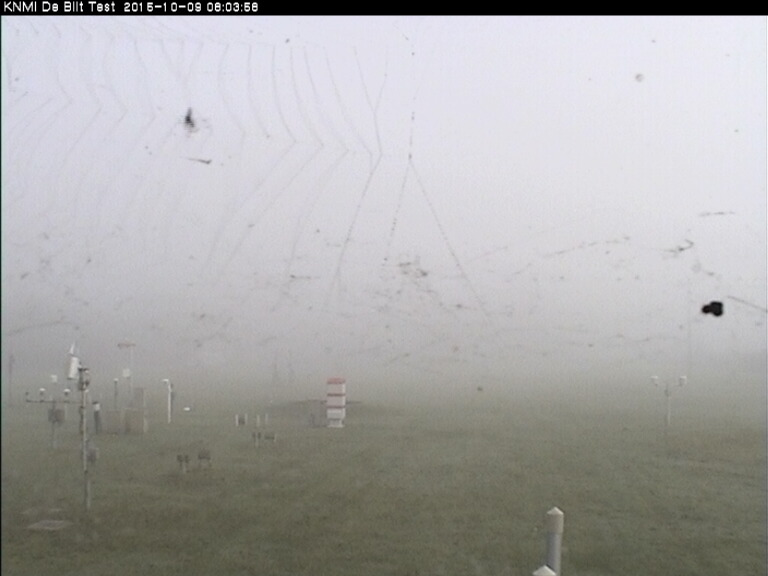
\includegraphics[width=0.22\textwidth]{Meetterrein_20151009_0800.jpg}	
			\caption{Measurement field at KNMI-De Bilt: fog conditions.}
			\label{fig:fog}
		\end{figure}

\section{Methodology}
The research starts with a literature survey to gain more insights in fog formation and pattern recognition in images to grasp the main points in the domain of application.
The main method to be used relies on the principles of pattern recognition and machine learning. 
First the work will focus to extract features indicating fog and mist in images. Such features are to be used to train a classifier. 
In few situations the problem can be considered supervised given the visibility information from a 
meteorological transmissiometer sensor (i.e., device able to measure the optical visibility) that acts as ground truth. However, the 
unsupervised definition of the problem should be considered as the standard condition. In general the features should primarily come from the image inspection, but it might be useful to also take into account meteorological parameters 
(temperature, wind speed, humidity, etc.) to be used as further features where
the information is available.

%\begin{figure}[ht]
%	\centering
%	\includegraphics[width=0.3\textwidth]{NeuralNetwork}	
%	\caption{Concept of a neural network with a single hidden layer. Several predictors are linearly combined into hidden units, which are transformed by a sinusoidal function. The hidden units are then combined linearly into a output \cite{Kuhn2013a}. }
%	\label{fig:NN}
%\end{figure}

\section{Expected Results}

A machine learning system that is able to classify the fog/mist conditions with high precision and recall
for the subset of samples that have a supervised approach and that is able to detect fog conditions in the unsupervised case. The approach found should be easily extensible to new camera images with 
minimal intervention in terms of parameters to be fed by the user.
Besides a report describing the research, we also aim at documented and reproducible code (likely available via Github).  

\bibliographystyle{IEEEtran}


\bibliography{biblio}



%\section{References}
%\begin{enumerate}
%	\item Kuhn, M., \& Johnson, K. (2013). Applied Predictive Modeling. \url{http://doi.org/10.1007/978-1-4614-6849-3}
%	\item \url{wow.knmi.nl}
%	\item \url{www.knmi.nl}
%	\item \url{wow.metoffice.gov.uk}
%\end{enumerate}
\end{document}